% !TEX TS-program = pdflatex
% !TEX encoding = UTF-8 Unicode

% This is a simple template for a LaTeX document using the "article" class.
% See "book", "report", "letter" for other types of document.

\documentclass[12pt]{article} % use larger type; default would be 10pt

\usepackage[utf8]{inputenc} % set input encoding (not needed with XeLaTeX)

%%% Examples of Article customizations
% These packages are optional, depending whether you want the features they provide.
% See the LaTeX Companion or other references for full information.

%%% PAGE DIMENSIONS
\usepackage{geometry} % to change the page dimensions
\geometry{a4paper} % or letterpaper (US) or a5paper or....
\geometry{margin=1cm} % for example, change the margins to 2 inches all round
% \geometry{landscape} % set up the page for landscape
%   read geometry.pdf for detailed page layout information

\usepackage{graphicx} % support the \includegraphics command and options

% \usepackage[parfill]{parskip} % Activate to begin paragraphs with an empty line rather than an indent

%%% PACKAGES
\usepackage{booktabs} % for much better looking tables
\usepackage{array} % for better arrays (eg matrices) in maths
\usepackage{paralist} % very flexible & customisable lists (eg. enumerate/itemize, etc.)
\usepackage{verbatim} % adds environment for commenting out blocks of text & for better verbatim
\usepackage{subfig} % make it possible to include more than one captioned figure/table in a single float
% These packages are all incorporated in the memoir class to one degree or another...

%%% HEADERS & FOOTERS
\usepackage{fancyhdr} % This should be set AFTER setting up the page geometry
\pagestyle{fancy} % options: empty , plain , fancy
\renewcommand{\headrulewidth}{0pt} % customise the layout...
%\lhead{}\chead{}\rhead{}
%\lfoot{}\cfoot{}\rfoot{}

%%% SECTION TITLE APPEARANCE
\usepackage{sectsty}
\allsectionsfont{\sffamily\mdseries\upshape} % (See the fntguide.pdf for font help)
% (This matches ConTeXt defaults)

%%% ToC (table of contents) APPEARANCE
\usepackage[nottoc,notlof,notlot]{tocbibind} % Put the bibliography in the ToC
\usepackage[titles,subfigure]{tocloft} % Alter the style of the Table of Contents
\renewcommand{\cftsecfont}{\rmfamily\mdseries\upshape}
\renewcommand{\cftsecpagefont}{\rmfamily\mdseries\upshape} % No bold!

%%% END Article customizations
\newcommand{\eqgood}{\overset{\surd}{=\joinrel=}}
\newcommand{\aufgabe}[1]{{\huge Statistik Übung \underline{Aufgabe #1}}\\[3.5ex]  } 
\usepackage{amsmath}
\usepackage{amssymb}
%%% The "real" document content comes below...

\usepackage{pgf-pie}

\begin{document}
\aufgabe{26}
Aufgabenstellung: \\
Glücksrad mit zwei Feldern rot und blau. Zwei Spieler drehen abwechselnd. 
Wenn der erste Spieler zuerst rot dreht, bevor der zweite Spieler blau dreht, gewinnt er. 
Wie groß müssen die Felder rot und blau sein, dass beide die selbe Gewinnchance haben? \\[0.5cm]
Lösung: \\
Zufallsvariable $X$: Wartezeit bis zur Entscheidung. \\
$P(X=1) = p$ und $P(X=2) = \overline{p}^2$\\
$p = \overline{p}^2 = p^2 - 2p + 1$\\
$p^2 - 3p +1 = 0$\\
$p_{1, 2} = \frac{3 \pm \sqrt{3^2 - 4 *1*1}}{2} = \frac{3 \pm \sqrt{5}}{2}$\\
$p = 38,2\%$\\[1ex]
Mit dem Gedächtnislosigkeitsargument folgt, dass die rote Fläche 137,5 Grad und die blaue Fläche 222,5 Grad groß sein muss, damit beide die gleiche Chance haben. \\
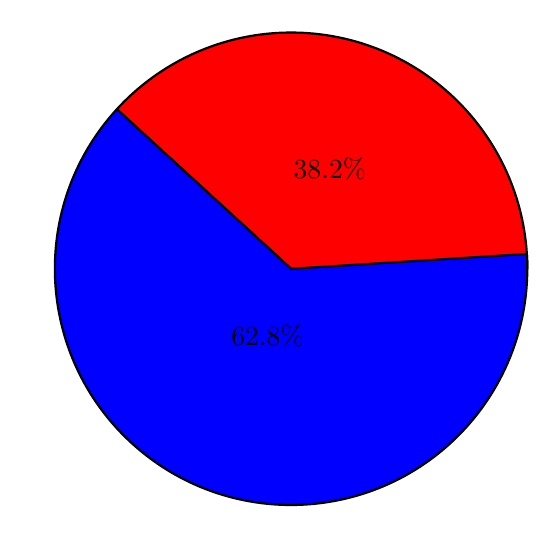
\begin{tikzpicture}
\pie[color={red, blue}]{ 38.2/ , 62.8/ } 
\end{tikzpicture}

\- \dotfill
\\[4ex]
\aufgabe{27}
Aufgabenstellung: \\
kumulierte Verteilungsfunktion $F_X(x) := 
\begin{cases}
0 
& \text{ falls } x<-2 \\
-\frac{3}{32}(x+2)(x-4) 
& \text{ falls } -2 \leq x<0\\
\frac{3}{4}
& \text{ falls } 0 \leq x<1\\
\frac{1}{60}x^4 + \frac{11}{15}
& \text{ falls } 1 \leq x<2\\
1
& \text{ falls } 2 \leq x\\
\end{cases}$\\
stetige Übergänge: \\
\begin{tabular}{rcl}
$0 = F_X(-2^{-})$ & $\eqgood$ &  $F_X(-2^{+}) = 0$\\
$0,75 = \frac{3}{4} = \frac{3 * 2 * 4}{32} = F_X(0^{-})$ & $\eqgood$ &  $F_X(0^{+}) = \frac{3}{4}$\\
$\frac{3}{4} = F_X(1^{-})$ & $\eqgood$ &   $F_X(1^{+}) = \frac{1}{60} * 1^4 + \frac{11}{15} = \frac{45}{60} = \frac{3}{4}$\\
$1 = \frac{1*2^4+44}{60} = F_X(2^{-})$ & $\eqgood$ &   $F_X(2^{+}) = 1$\\
\end{tabular}\\
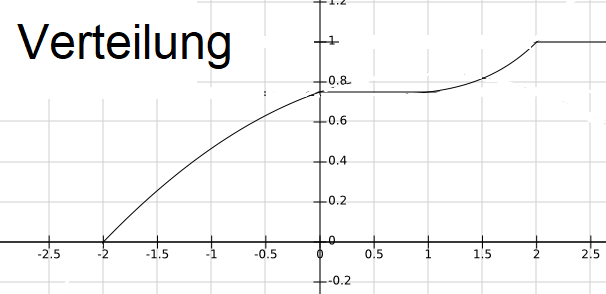
\includegraphics[scale=1]{A27F.png}\\
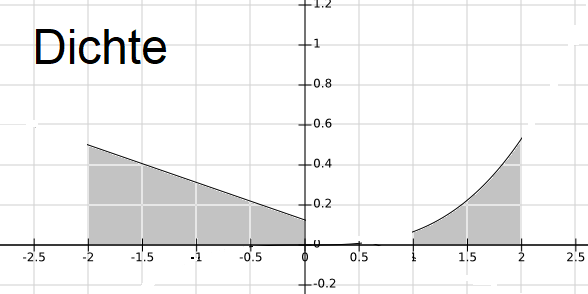
\includegraphics[scale=1]{A27D.png}\\
Dichte $\rho_X |_{\ldots} = \frac{dF_X | {\ldots} (x)}{dx} = 
\begin{cases}
0 
& \text{ falls } x<-2 \\
-\frac{3}{32}((x+2)+(x-4)) = \frac{-3x + 2}{16}
& \text{ falls } -2 < x<0\\
0
& \text{ falls } 0 < x<1\\
\frac{1}{15}x^3
& \text{ falls } 1 < x<2\\
0
& \text{ falls } 2 < x\\
\end{cases}$\\
rechtsstetige Dichtefortsetzung: \\
Dichte $\rho_X |_{\ldots} = \frac{dF_X | {\ldots} (x)}{dx} = 
\begin{cases}
\frac{-3x + 2}{16}
& \text{ falls } -2 \leq x<0\\
\frac{1}{15}x^3
& \text{ falls } 1 \leq x<2\\
0
& \text{ sonst } \\
\end{cases}$\\
$1/3$-Quantil: $1 / 3 = F_X(x_{1/3}) = -3/32 * (x_{1/3} + 2) * (x_{1/3} - 4) = -3/32 * (x_{1/3}^2 - 2 * x_{1/3} - 8)$\\
$0 = \frac{-9}{32} (x_{1/3}^2 - 2 * x_{1/3} - 8) - 1 $\\
$0 = 9 x_{1/3}^2 - 18 * x_{1/3} - 72+32$\\
$x_{1/3} = \frac{18 \pm \sqrt{18^2+4*9*40}}{18} = 1 \pm \frac{\sqrt{1768}}{18} = 1 \pm \frac{42}{18} = 1 \pm \frac{7}{3}$\\
$x_{1/3} = \frac{-4}{3} \qquad \qquad \surd \text{durch Graphik bestaetigt. }$\\[1ex]
$P(X=1/2) = 0$ \\[1ex]
$P(-1 \leq X \leq 3) = F_X(3^{+}) - F_X(-1^{-}) = 1 - \frac{-3*1*(-5)}{32} = 1-\frac{15}{32} = \frac{17}{32} = 53,125\% $\\[1ex]
\newpage
\aufgabe{28}
$\overline{D} = 1.100,85 $\\
$\overline{D^2} = 1.218.115,55 $\\
$\overline{T} = 59,82 $\\
$\overline{T^2} = 4.156,7 $\\
$\overline{DT} = 67.742 $\\
Empirische Kovarianz $s_{DT} = \overline{DT} - \overline{D} * \overline{T} = 67.742 - 1.100,85 * 59,85 = 1.889,153$ \\
Empirische Varianz $s_{D}^2 = \overline{D^2} - \overline{D}^2 = 1.218.115,5 - 1.100,85^2 = 6.244,778$ \\
Empirische Varianz $s_{T}^2 = \overline{T^2} - \overline{T}^2 = 4156,7 - 59,82^2 = 578,268$ \\[1ex]
Korrellationskoeffizient $r_{DT} = \frac{s_{DT}}{s_{D}s_{T}} = \frac{1.889,153}{\sqrt{6.244,778 * 578,268}} = \frac{1889,153}{1900,303} = 99,413 \%$\\[1ex]
Regressionsgeradensteigung $g' = \frac{s_{DT}}{s_{D}^2} = \frac{1.889,153}{6.244,778} = 0,30$\\
Regressionsgeraden-y-Achsenabschnitt $g(0) = \overline{T} - g' \overline{D} = 59,82 - 0,30 * 1.100,85 = -273,206$ \\
\begin{tabular}{|r|r|r|r|}
\hline
empir. Druck & approx. Temp & empir. Temp & rel Fehler \\ \hline \hline
990,9 & 26,558 & 25 & 6,2\%\\ \hline
1.008,5 & 31,883 & 30 & 6,3\%\\ \hline
1.023,4 & 36,390 & 35 & 4,0\%\\ \hline
1.035,6 & 40,081 & 40 & 0,2\%\\ \hline
1.064,0 & 48,672 & 50 & -2,7\%\\ \hline
1.095,2 & 58,111 & 60 & -3,1\%\\ \hline
1.126,3 & 67,519 & 70 & -3,5\%\\ \hline
1.153,4 & 75,717 & 80 & -5,4\%\\ \hline
1.177,8 & 83,099 & 85 & -2,2\%\\ \hline
1.207,6 & 92,114 & 90 & 2,3\%\\ \hline
1.226,6 & 97,862 & 93 & 5,2\%\\ \hline
\end{tabular}\\
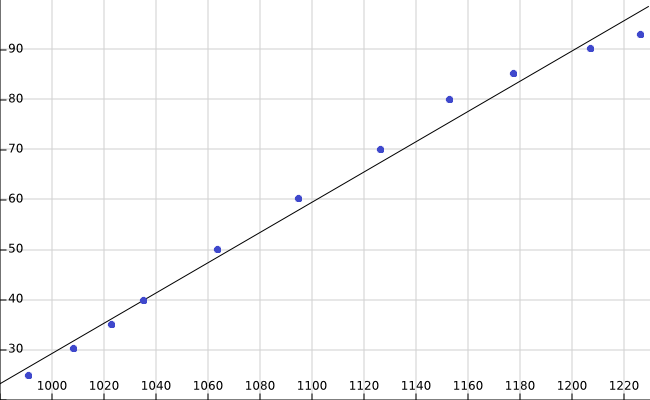
\includegraphics{A28.png}\\

\end{document}
